%!TEX root = thesis.tex
\chapter{Background Studies}
\section{Caches}
Solely, a cache is a small, fast, array of memory which is placed between lower level memory and higher one.  It store a special block of information, in order to increase performance of computer systems. It is like a buffer area which has some logic to exploit locality features of programming logic. Today, with increasing of processing ability of computer systems, memory access is bottle neck. 

The "cache" is originally french rooted with meaning "concealed place for storage."\cite{sloss2004arm} We can move this definition basically to the computer science. The cache's design is definitely  isolated from software layer, however; if you know your caches feature and how caches working you could program a lot more efficient codes easily.



\subsection{Motivation of Caches and Principle of Locality}
The main motivation of caches is indisputably performance. As we mentioned,  Performance of high-speed computers is usually limited by memory bandwidth and latency. In order to increase, and turn around that, we use an small array of memory which is located close to the processors.  The location of chip is important and there are many design decision (e.g On chip, out of chip), but more crucial  properties of caches are their designs (e.g. Naive Capacitor , SRAM, DRAM) and their logic complexity\cite{hennessy2012computer}.Due to physical constrains, the size of the memory is limited which we can locate close to memory. On the other hand, these design choices are decisive factor about prices of memories.  Because of all these reasons, Multi-Layer Memory Hierarchy with several caches  between processor core and main memory is well-known option in order to improve performance. Nevertheless, In multilayer memory hierarchy, it is hard to know where the particular data reside in, and whether it is coherent or not. It also add many layer between memory and processor and in some cases it even decrease system performance,especially because of logical complexity of the line.

The idea all the caches logic depending on is Principle of Locality. Principle of locality is actually a concern of information theory\cite{shannon2001mathematical}. It a conjecture of data distribution and processing order. The phenomenon assume that the the same data and related document will be accessed more frequently than other data\cite{denning2005locality}. Today, it is the one of the corner stone of computer science.  It was first developed with Atlas System with purpose to develop virtual memory systems work well\cite{kilburn1962one}. Then, it spread from search engines optimization to hardware caches. 

\begin{figure}[h!]
    \centering
    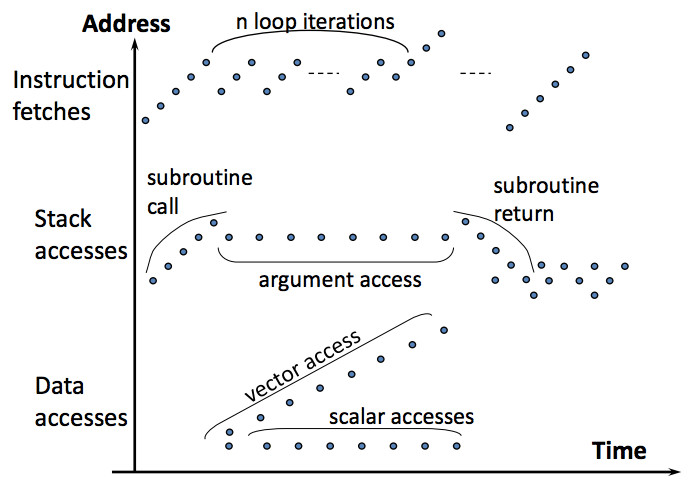
\includegraphics[width=1\textwidth]{img/localitygraph2.jpg}
    \caption{Principle of Locality}
    \cite{ComputerArchCoursera}
    \label{fig:principleoflocality}
\end{figure}


There are mainly two type of locality of reference:

\begin{description}
\item[Spacial Locality] Spacial locality propose if there is a particular of memory which is accessed on memory, then it is more likely to accessing memory locations around of it in near feature. Especially arrays and instructions are exploiting this locality. Arrays, formed structure and instructions on memory are laid out lineally over memory. On figure \ref{fig:principleoflocality}, we can see spacial locality simply.  For example, during instruction fetches part on the figure, n loop iterations accesses same memory locations for many times.  There are also subclass of spacial localities like Branch Locality and Equidistant Locality. They are designed locality types of indeterministic feature of program structure. Branch prediction and Special compiler designs aims to exploits this kind of locality more efficiently.
\item[Temporal Locality] Temporal locality propose if there is a particular of memory location which is accessed recently, it will be accessed again more likely than any other location. Especially, variables, subroutines of stacks or other calls exploits this feature of locality. On figure \ref{fig:principleoflocality}, it is obviously seen that the values accessed once is possible to accessed again. 
\end{description}

\begin{figure}[h!]
    \centering
    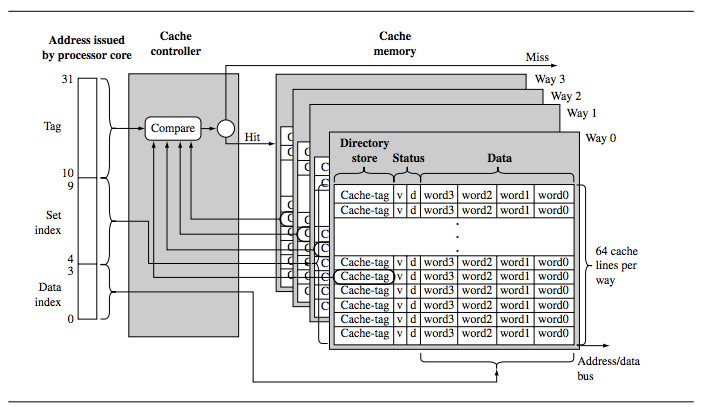
\includegraphics[width=1\textwidth]{img/cacheinternals.jpg}
    \caption{4 KB 4-way set associative cache with 256 cache lines }
    \cite{sloss2004arm}
    \label{fig:cacheinternals}
\end{figure}

\subsection{The basic logic of caches}
As we said in previous section, the basic logic behind caches is moving arranging caches with local data. In order to provide this feature as smooth as possible, we use a logic circuit called "Cache Controller". It does basic logic comparison and wiring the request and response into the right path. Thus, it intercept the write and read request from processor, replace its memory array with right scheduling method, and evict it safely and coherently. It processes with diving address of th request into three fields which are  Index set field, tag field, and block field. In figure \ref{fig:cacheinternals}, these fields showed. 

At the beginning of cache process after it divided address fields, It first request right cache line which is shown in figure \ref{fig:principleoflocality}. So if we have $M$ byte memory and $N$ byte cache line, we must have $M/N = cache line$, then we can represent it with $p$ when $cache line = 2^{p}$ Thus, cache controller just wire corresponding line with given set index. 

In traditional cache convention, first field belongs to tag id. Tag id is determined depending on other field i.e. the remaining part after index field and block field calculated is tag id length. Tag id is using to verify the stored line is actually belongs to right location of memory. The cache controller has comparison circuit(XOR) and compare the requested address and the address which is in the pointed line by set index field. If they are matched with each other, then it check valid byte and hit or miss. There is a simple AND circuit between tag comparison. 

Final field is called data index or block index field. It will point in the cache line the smallest addressable memory location. Therefore, when processor want to read a value, cache fetch the whole block, and that makes cache to exploit spacial locality linearly. However, it will limit the access speed remarkable, if we increase block size. The optimum block size is about 64 byte for many system. As we mention before each cache line includes cache-tag field, valid bit, dirty bit, and some coherency bits in some special systems. The length of the data index field is equal to r if  $ word size = 2^{r}  $.

When we increase the set index count it increase basically temporal locality, but not always. The cache conflict could happened when two memory location which uses same cache line could be used concurrently or twisted. Highly trashing can reduce cache performance. For this reason, associative caches are developed. Set associative caches are represented by their way number e.g 3 way associative caches or full associative caches, and there are group of cache arrays corresponding to the same set index. So that decrease the set index count but increase the performance during conflict miss in some cases. However, because of the complexity of the comparison circuit, it must be carefully chosen the number of ways. The associative caches are showed in figure \ref{fig:cacheinternals}. 

The computer architecture we uses today actually first formulated by John Von Neumann  \cite{von1961collected}. On the first design of computer it was a single cycle instruction machine without any pipeline or superscalar idea. Then Hardward Mark I machine is designed with proposing two type of caches which are one for instruction, and one for data. Icache and Dcache are specified for their own purpose, because data and instruction on memories have different deterministic properties. Instruction are more tent to be linearly accessed by memory and they has branch locality which can be predict earlier. Icache also could be located more close to decode and fetch parts of processors when Dcache are instead closer to memory fetch parts. Yet, the most significant benefit of Harward design is concurrently usage both caches during pipelined architectures. 
\subsection{Allocation, Write and Replacement Policies}
There are three policy type determine a cache behaviours. They are write policy, read policy and reallocate policy. System's performance, coherency, and designs are determined depending on these rules. 

\begin{figure}[h!]
    \centering
    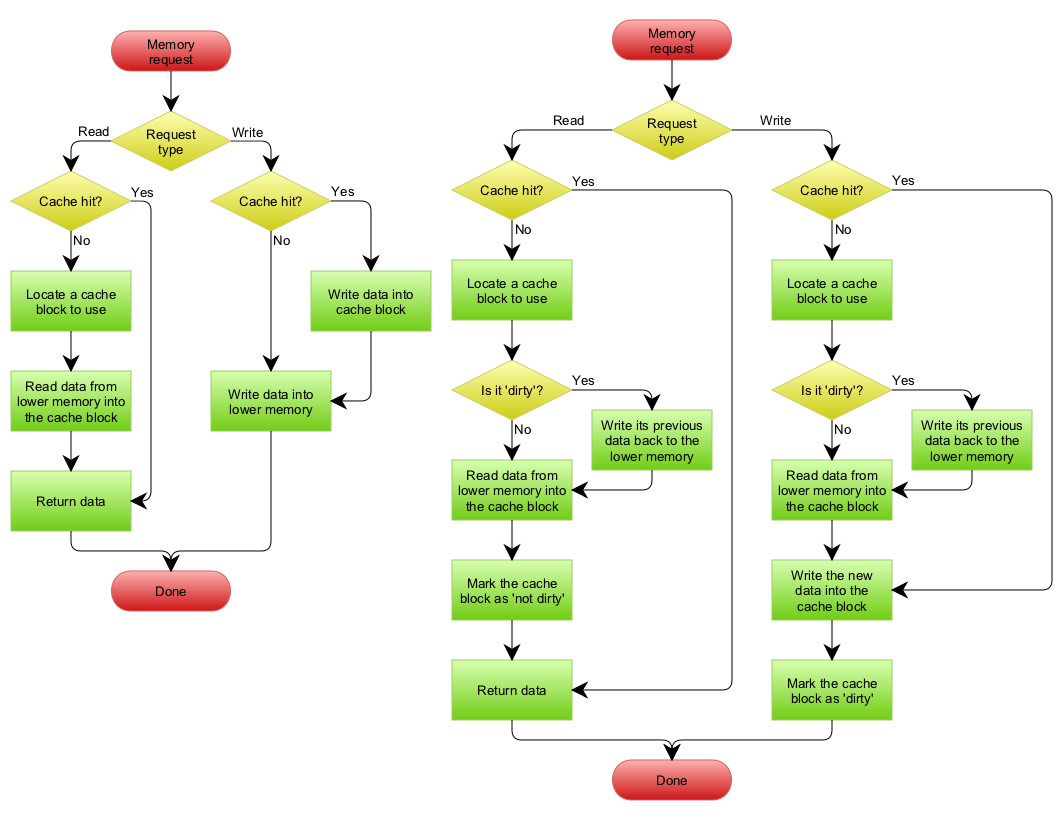
\includegraphics[width=1\textwidth]{img/policies.jpg}
    \caption{A. A Write-Through cache with No-Write Allocation B. A Write-Back cache with Write Allocation}
    \cite{wikipolicies}
    \label{fig:cachepolicies}
\end{figure}

\subsection*{Write Policies }
\begin{description}
\item[Write Through] When the cache controller designed based on $write through$ policy, it write the values into the memory and caches simultaneously, when the write request is arrived from processors. It does not depend on $write miss$ or $write hit$. It will reduce write performance, because writing data on memory is a lot slower, but it stay coherent all the times. It is performance could be increased a bit  with write buffer memories between memory and cache.
\item[Write Back] The systems with that policies does not have same values in memory and corresponding cache line, so the coherency between memory and caches are provided by a trashing algorithm. Cache line always store more recent data, but if there is more than one cache it is hard to decide which one is more valid or whether there is a valid coherent one.  However, it effects performance quite remarkable (e.g. in ARM 15 cpu writing cycle to memory is around 200 cycle, but caches is about 4.) . The system with limited register numbers can overflow to the memory to store loop variables and that could increase write memory usage. $Write Back$ policy makes this kind of systems really effective. The dirty bit are stand for $WriteBack$ policy. If you write some value on any cache line, dirty bit must be set for eviction. During trashing process, you must first move dirt block back to memory. 
\end{description}
\subsection*{Replacement Policies }
\begin{description}
\item[Random] Random policies are designed to evict a random line in the associative caches. It is  not really random on implementation, but enough random to work with it. It sounds to weak and primitive approach but actually it could be really effective on highly associative caches. 
\item[Least Recently Used ] Least recently used replacement policies are actually implemented in two types. Fully most recently used and Not most recently used random. It is probably the most efficient algorithm to replace cache index sets, but it is really hard to implement on highly associative caches. You must record history of schedule and update it each attempt of access. It could be most effective and easy method on 2 way associative caches and it just need one bit to record who used last. It actually increase temporal locality, because it offers the most recently used one is more likely to be used again. The most recently used but random is a hybrid solution of least recently used and random policies. It just record who accessed last and replace one random set except most recently one. 
\item[First In First Out] It is also known Round robin. It is also mostly using with highly associative caches. In its implementation, it has one one tail pointer of stack and in each attempt of access it evict tail pointers set, and increment the the tail pointer to next set. 
\end{description}
\subsection*{Allocation Policies }
\begin{description}
\item[Write Allocate] $Write Allocate$ policy is also known as $Read Write Allocate$ policy. It refers that during write miss process, cache controller allocates the cache line with related address, as like as normal read miss process. It is mostly using with $WriteBack$ policies, because it assume it is more likely to access same data which you write before. 
\item[No-Write Allocate] $No-Write Allocate$ policy is also known $Read Allocate$. It is an exotic implementation of caches. It is generally seen with $WriteThough$ policy. This systems can be special to read privileged and they do not hope to read or write subsequent write(or even read after write.) 
\end{description}

\subsection{Miss Type and Advance Cache Optimization Methods}
\subsection*{Miss Type}
\begin{description}
\item[Cold Misses]  Cold misses are sometimes referred to as compulsory misses . If you never invoke related memory address and if you calling it first time,  You will encounter with that misses. It is natural misses, and really hard to mitigate them. Spacial locality is the one of the method to avoid this misses. As we mention before, when we increase the size of block, it will increase spacial locality.Also before initializing memory, pre-fetching algorithms and branch prediction algorithms can be useful to eliminate this kind of misses. In addition to this, usage of large amount of caches will naturally reduce this misses, but it is side effect of it.
\item[Conflict Misses] Those misses are the one we are able to avoid. Conflict happens in systems set with lower associativity esp. with direct map systems. To reduce this you should increase associativity. In full associative caches, it all conflict misses are avoided. The change of conflict miss is $tagsize/memorysize$.
\item[Capacity Misses] They are also natural misses related with size of the caches. We can not store every information in memory into cache. Those misses are based by definition of caches.  You can't solve it even with perfect replacement algorithm, but maybe you could decrease the rate of capacity miss with pre-fetching.
\end{description}
\subsection*{Advance Cache Optimization Methods}
\begin{description}
\item[Pipelined Caches] As we did in processors, we could divide cache organization in two separate stage which are decode and data. It will increase the writing efficiency because it will increase the bandwidth during subsequent requests. However the clock mechanism will decrease to hit time.  
\item[Write Buffers] Write buffers are small fully associated buffer memories between caches and memories. They effects cache performance because the time between writing values to memory from cache, cache memories must lock if we do not use cache memories. Thus, Cache memories store values to buffer buffer will responsible with writing it. Buffer size is important, when consecutive write operation requested. When buffers is full, it will makes cache lock to get empty.
\item[Multilayer Cache] Multilayer caches are game changer optimization decisions, because when we have level 2 caches, then we could have faster level 1 caches, because it could be smaller and simpler. Namely, we are adding systems higher level caches, in order to, decrease lower level caches miss time penalty and increase the hit response time, but it will decrease lower level caches hit rate. Level 2 or higher caches could be also on-chip (i.e fast as possible) and SRAM, yet lower level caches must always be faster closer and simpler.
\item[Victim Caches] Victim caches are really useful and simple idea for decreasing miss penalty time. It is a buffer memory, fully associative and mostly 4 to 16 cache line. It stores recently evicted lines in it. It means it increase the associativity of recently used lines on other small buffer with cheap and flexible design.
\item[Hardware Prefetching] There are many theoretical pre-fetching method, but there are a few example implemented. The most well known is prefetch the most recently values incremental block line. That targets to increase most recently used ones spacial locality. It is really efficient to applying it, because increasing block depth is expensive job for caches and increase hit time. If you implement one buffer memory, which prefetch next block of block you need, it automatically increase spacial locality. Also compiler based branch prediction methods are good example of instruction prefetching, however, generally, prefethers for instruction caches load all branches to decrease miss rate.
\item[Non-Blocking Caches]
\end{description}
\section{Cache Coherence and  Consistency}
Many modern computer systems with parallel processing ability have support of shared memory in hardware. Shared memory has lots of advantage over message based memory systems.  Each processor could access same address space, read and write them simultaneously with using their own caches. This features has lots of benefit such as; low power consumption, higher performance and lower prices. However, without consistency between processors, parallel processing can not use many advantage of parallel programming. It could be also insecure to use a system without consistency between processors. 

To provide better understanding of shared memory correctness, we defined it in two separate them in two definition, which are consistency and coherency. Consistency provide a definition of memory access rules and how they will act around computer system with store and load operations. When we compare it with coherency model, it must be more simple and easy to understand it. Therefore, it define a correct behaviours of the memory accesses of multiple threads by allowing or disallowing executions. On the other hand Coherency is a way of implementing a control protocol between memories and processors to support and provide consistency. Correct coherency provide a system which programmer or operator of the system can never determine behaviours (misbehaviours or correct behaviours) of caches\cite{sorin2011primer}.

As mentioned, Mention Consistency is try to define to correct shared memory behaviour between many processor in term of loads and stores. It does not have to concern specific hardware issues, such as hardware level pipelines, write buffers, caches, Out-of-order processing schemes etc. However, in the market, there is no hardware provide consistency perfectly, because the reordering store and load operations is regular optimization techniques in out-of-order processors. In addition to out-of-order processors, the multi layer memory architecture makes consistency vague and subtle. Yet, most of the programmers assume memories are completely consistent. There are several level between inconsistent and sequentially consistent memory. 

\todo[inline]{Mention Consistency Application Summery.}

\begin{figure}[h!]
    \centering
    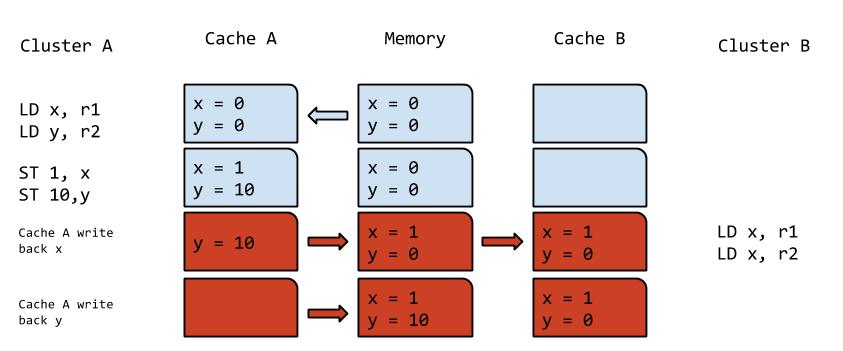
\includegraphics[width=1\textwidth]{img/cacheinconsistencywriteback.jpg}
    \caption{Write-back Policy Cache Memory Inconsistency}
    \label{fig:cacheinconsistencywriteback}
\end{figure}

Memory Coherency (a.k.a. Cache Coherency) is actually to impose a protocol between caches to provide a specific consistency model on shared memory systems. Unlikely consistency, it also concern hardware uncertainness and 
subtle part such as write buffer, pre-fetcher. Typical consistency protocol has features which include instruction caches, multiple-level caches, virtual-physical address transaction, and coherent direct memory access. However, it is not enough to ensure consistency(depending on consistency model) by itself. It tries to makes caches synchronization in shared memory systems invisible from software developer. However there are timing techniques to analysis cache architecture and coherency model of system. 

In figure \ref{fig:cacheinconsistencywriteback} and \ref{fig:cacheinconsistencywritethrough}, the consistency issues on multi layer memory systems. Assume there is two cluster which has ability to process values with given instruction codes. LD and ST instruction refer to memory load and store request. In figure \ref{fig:cacheinconsistencywriteback}, there is a system with two caches which belongs each cluster and one shared memory block. x and y is represents a particular memory address. Contrast with figure \ref{fig:cacheinconsistencywritethrough}, figure \ref{fig:cacheinconsistencywriteback} uses write-back policy. In step 1, cluster A loaded x and y to the processor(it could be also pre-fetcher who load them to the cache block). In second step, somehow clusters stored 1 in memory location x and 10 in memory location y. In this step, memory is not consistent with memory but it is not hazard because they are not shared with cluster B. In step 3, caches evicted the block which include address x and later address x and y were loaded into the cache B. After this moment, they will never share the values which other cluster is actually using. Y was 10 at the end in the memory but it can't be seen by cluster B, even if it try to read it a million times. 


\begin{figure}[h!]
    \centering
    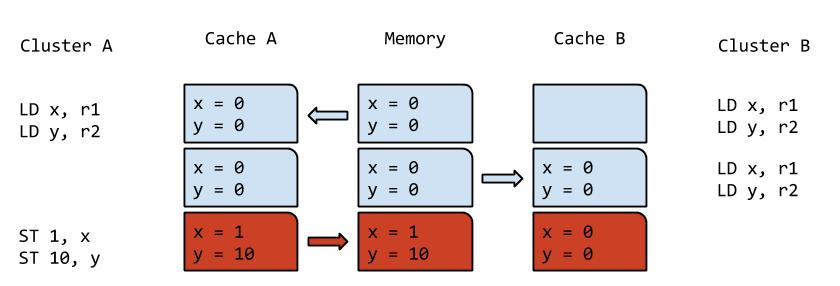
\includegraphics[width=1\textwidth]{img/cacheinconsistencywritethrough.jpg}
    \caption{Write-through Policy Cache Memory Inconsistency}
    \label{fig:cacheinconsistencywritethrough}
\end{figure}

Write-through cache policy is intuitively perceived as solution of this problem, because it just write every values directly to the memory and it will be always synchronized with memory, yet it is not. In figure \ref{fig:cacheinconsistencywritethrough}, write-through cache policy inconsistency showed. The problem with write-through policy, clusters use values which in their cache instead of memory, so even if memory is consistent with clusters, it is not consistent with each caches. In step 1 of figure \ref{fig:cacheinconsistencywritethrough}, cluster A loaded x and y addresses into the its registers. Then, in step 2, cluster B loaded  values of x and y addresses. In step 3, system got in inconsistent state, because cluster A write values through memory, but Cluster B uses the old values, and it will never reach never values, even if it try to load many times. For this reason, many of the large systems which has more than 64 core use this type of cache coherence.

In order to solve this problems, there are several coherency mechanisms and their protocols.  Depending on the case and the number of cluster or processor in the system, system could use Snooping and Directory based mechanism. These each protocol have their own benefits and drawbacks. Snooping protocol is tent to use a lot of bandwidth, however, it is faster and more synchronous. Its logic is to broadcast each state to every node on the system. However, directory based mechanism work with request and response. There is interconnector to forward message to the right address and it makes directory based mechanism slower because of the increased latency, lighter because of the decreased bandwidth.

\subsection{Snooping Coherence Protocols}
Snooping coherence (a.k.a. Bus Sniffing) is a technique to have caches to watch other processors caches and provide consistency depending on specified protocol.  It basically implemented with external port to the system bus. Therefore, it implemented over cache controller which has feature to watch bus. It makes cache controller bigger and waste more power, so lower layer caches could use less complex coherency protocols and vice versa. There are many snoopy cache coherency protocol also depending on consistency model, but we can categorize them in two class which are Write update and write invalidate. 

In this both protocol, we try to get rid of stall data which are in different caches, but it is provided with different logics. Write-update protocol is a broadcast write protocol that in every write attempt, it will write the values into the corresponding cache block but also it broadcast the write message to the every caches on the connected bus. Thus, everyone on the bus which has the ability of interpreting the message of write-update protocol will update stall values with new ones. 

Secondly, Write-invalidate is whenever you write, you invalidate other cache copies and reduce to possibility usage of stall data. Instead of sending whole data block, it just send the tag number and state of the tag. It could effectively be successful, if you have limited bandwidth and power source. Most processor with coherency is today using write-invalidate protocol. However, it is efficient if there a few writer and many reader clusters or processors. Comparing with write-update protocol, if there is many writer, it could be less efficient because of invalidation process validate-invalidate-forward hops.\cite{ComputerArchCoursera}

There are many protocols for both write-invalidate and write-update to maintain coherence, such as MSI, MESI (aka Illinois), MOSI, MOESI, MESIF, write-once, and Synapse, Berkeley, Firefly and Dragon protocol. In this thesis, we will just focus on write-invalidate protocols because of their popularity, but basic principles are same as each other.

\todo[inline]{Mention Serialization of buses}


\subsubsection{MSI - Basic}

\begin{table}[position specifier]
\centering
\begin{tabular}{|c|c|c|c|c|}
\hline 
• & Clean/Dirtiy & Write? & Unique? & Silent Transition to \\ 
\hline 
Invalid & Clean & No & No & - \\ 
\hline 
Shared & Clean & No & No & Invalid State \\ 
\hline 
Modified & Dirty & Yes & Yes & - \\ 
\hline 
\end{tabular} 
\caption{MSI states' properties}
\label{tab:MSItable}
\end{table}


Basic write-invalidate snoopy cache control protocol is MSI (a.k.a Modified-Shared-Invalid protocol). In this model, each cache block has cache tag, and two status bit as same as standard caches, but instead of dirt and valid status bit, MSI cache line has state bits to refer in which state it is. MSI has three state in state machine and they are "Modified", "Shared", "Invalid". two bits can represent four state, so definitely represent three state. The main idea behind this protocol is that one writer and many reader states provide always consistent memory sharing. Therefore, every cache in the system has different responsibilities when they read or write.

\begin{description}
\item[Invalid] Invalid state is exactly same state with standard caches' invalid state. When cache need to access a invalid block, it must act as cache miss, and  be fetched this block again.
\item[Shared] When there is no writer processor on this line, and if  a processor request this line with purpose of read it, it will be in shared state.  It is read-only cache block, and processors are not allowed write without transforming state. The processor also can evict it without writing back to the upper layer memory, because that is for sure, it is clean block.
\item[Modified] It is modified and also modifiable cache block. In a memory coherent system there can be at most one modified cache and all other cache must be invalidated. It is responsible with writing back cache to the upper layer memory. 
\end{description}


\begin{figure}[h!]
    \centering
    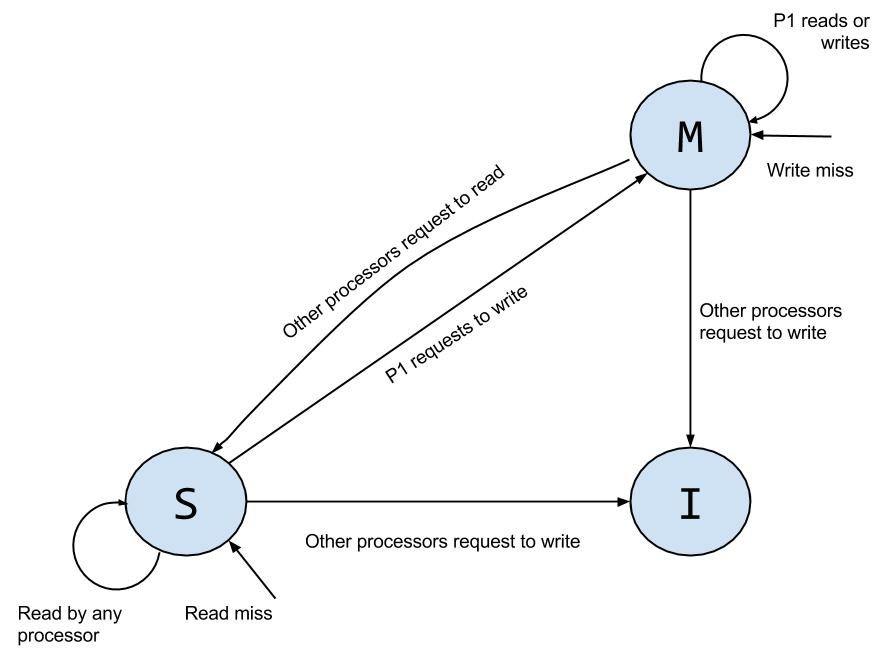
\includegraphics[width=1\textwidth]{img/MSIstatediagram.jpg}
    \caption{MSI State Diagram for processor P1}
    \label{fig:MSIstatediagram}
\end{figure}

In figure \ref{fig:MSIstatediagram}, MSI protocol's state diagram is showed. Cache memory launch with invalid cache block, and when a read miss is comprised,  cache controller will request memory block from memory. Then, the snooping control bus will broadcast the request of read. If there is a modified copy on the bus, it will abort request of memory block from memory. It will evict its line to memory, and change its state to shared state. Then, memory responds source of the request. After the fetching cache block to the source cache it, it sets the state as shared state. If there is a shared stated copies in the system, It does not matter who responds the request. In any case, It will fetch the memory block, and sets the state bits to shared.

When write miss is compromised in invalid state or shared, It will fetch the data as same as read miss cases, but the difference is it will invalidate other case's corresponding block which are shared or modified. Modified stated block must evict blocks properly. At the end, source cache block fetches the block.

Write hit can be compromise in modified state, and read hit can be compromise in shared state.

\subsubsection{MESI - Exclusive}
\begin{figure}[h!]
    \centering
    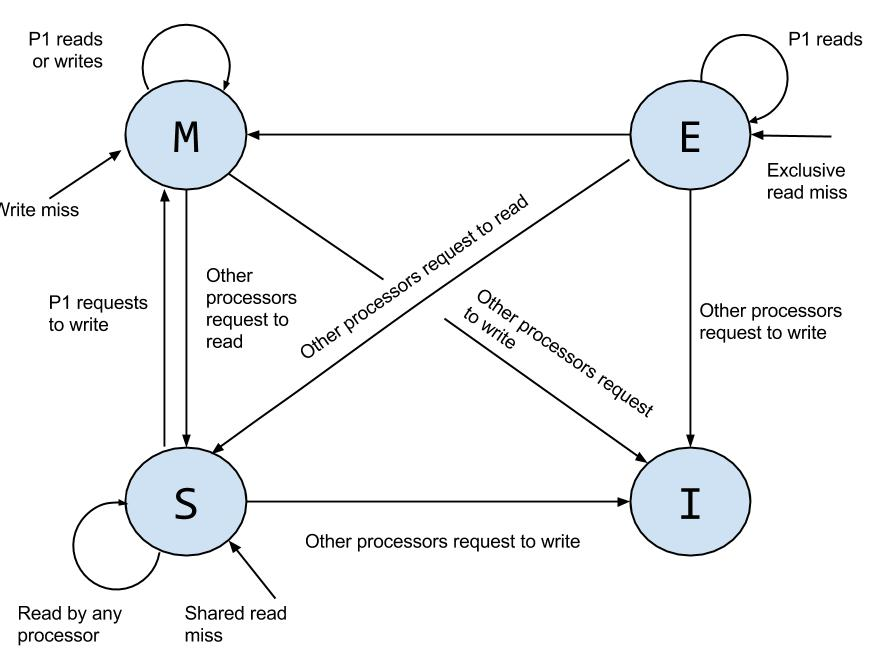
\includegraphics[width=1\textwidth]{img/MESIstatediagram.jpg}
    \caption{MESI State Diagram for processor P1}
    \label{fig:MESIstatediagram}
\end{figure}


The MESI protocol (a.k.a Illinois protocol due to its development at the University of Illinois at Urbana-Champaign) is a widely used cache coherency protocol\cite{papamarcos1984low}. The idea behind the MESI is to use forth state we can use with 2 bits. In order to increase efficiency $exclusive$ state is developed by JH. Patel et. al. in 1984\cite{papamarcos1984low}. As showed in MSI protocol, there is modified, shared and invalid states but also we have exclusive state. This exclusive states also known unmodified exclusive state, if we refer modified state as modified exclusive. This is very similar to the shared state in MSI, and in fact, Shared state is split in two different states. That is because of reducing the communication on the bus and increasing efficiency. In this case, there is exclusive cache blocks which are in read mode and they are unique i.e there is no other cache controller on the system has this cache block. 

\begin{description}
\item[Exclusive] The cache line is only present in current cache memory, and it has not modified yet. It is not a state to provide coherency, but it is state for increasing efficiency of bus bandwidth usage. When a cache line in exclusive state the cache controller can decide the transaction of the line without communicating with other caches. When a cache is requested with load operation, it is loaded in exclusive state, if there is no other cache controller has the cache block.
\end{description}


\begin{table}[position specifier]
\centering
\begin{tabular}{|c|c|c|c|c|}
\hline 
• & Clean/Dirtiy & Write? & Unique? & Silent Transition to \\ 
\hline 
Invalid & Clean & No & No & - \\ 
\hline 
Shared & Clean & No & No & Invalid State \\ 
\hline 
Excursive & Clean & No & Yes & Shared Modified Exclusive States \\ 
\hline 
Modified & Dirty & Yes & Yes & - \\ 
\hline 
\end{tabular} 
\caption{MESI states' properties}
\label{tab:MESItable}
\end{table}

In figure \ref{fig:MESIstatediagram}, state transactions are showed. Bus usage is bottle neck, low performance behavior in cache coherency. Silent state transactions are transactions in cache controller without communicating with other caches. For example, there is no need to broadcast and occupy bus for invalidating shared state in MSI protocol. If a cache controller is in shared state, the other cache controller can be shared or invalidate in MSI, so there is no dependency in the system transaction from shared to invalidate. Exclusive state is to exploit the salient transactions. When a load request arrive to cache controller from a processor, it request the line from upper level memory controller and other child caches controller. If any child controller send a shared state broadcast message, it load it in shared state. If there is a exclusive cache controller on the bus, it will degrade its state to shared and broadcast it. If there is no other shared state on the bus. It load the cache line in excluded state. Then, in case of store operation from processor, it will transact its state from exclusive to modified. It does not need to broadcast it, because we know it is unique in system. Contrast with modified state, due to be cleanness of the line, it does not need to evict line to upper memory, it can  just invalidate it silently. The weakness of this protocol comparing with MSI, if there is many processor with the corresponding cache line, when it count the copies to test uniqueness, it occupy shared bus more in some cases. If there is n cache controller with corresponding cache line, it will send n broadcast message with this message, however, instead of sending whole line to upper memory it is mostly efficient to send this message.

\subsubsection{MOESI - Owned Exclusive}
\begin{figure}[h!]
    \centering
    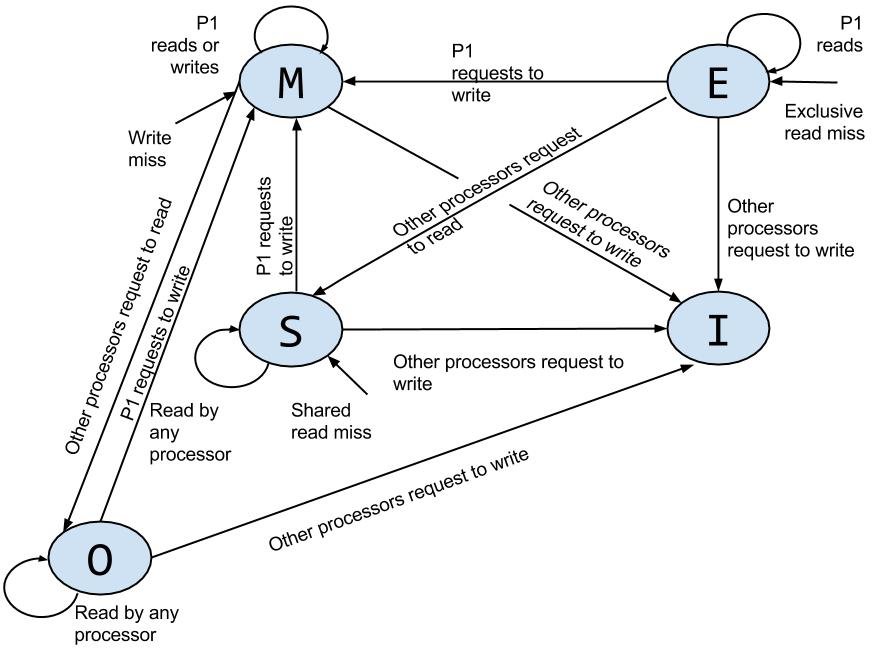
\includegraphics[width=1\textwidth]{img/MOESIstatediagram.jpg}
    \caption{MOESI State Diagram for processor P1}
    \label{fig:MOESIstatediagram}
\end{figure}

\begin{table}[position specifier]
\centering
\begin{tabular}{|c|c|c|c|c|}
\hline 
• & Clean/Dirtiy & Write? & Unique? & Silent Transition to \\ 
\hline 
Invalid & Clean & No & No & - \\ 
\hline 
Shared & Either & No & No & Invalid State \\ 
\hline 
Excursive & Clean & No & Yes & Shared Modified Exclusive States \\ 
\hline 
Owned & Dirty & No & Yes & - \\ 
\hline 
Modified & Dirty & Yes & Yes & Owned \\ 
\hline 
\end{tabular} 
\caption{MEOSI states' properties}
\label{tab:MOSItable}
\end{table}

Such processor producers AMD Opteron and Arm Cortex A are using MOESI protocol for cache sharing. In addition to the four states in MESI, a fifth state "Owned" appears here representing data that is both modified and shared. Using MOESI, instead of writing modified data back to main memory, it directly forward the dirty value from cache to cache before being shared, which could save bandwidth and gain much faster access to users to the cache.

\begin{description}
\item[Owned] Owned state is a state if and only if a cache line can transact in it, when a read request message snooped from another processors when the cache line is in modified state. It allows dirty line sharing between caches, and reduce the latency which is arisen due to the communication between memories and processors. The line is read only by all processors, when it is owned state.
\end{description}

In figure \ref{fig:MOESIstatediagram}, state transactions of MOESI protocol are showed. The relationships of states are almost same with MESI, but there is a state which supplants upper level memory with its own cache line. Hence, it is responsible with evicting lines and cleaning state. The cache line may be changed to the Modified state after invalidating all shared copies, or changed to the Shared state by writing the modifications back to main memory. If could increase efficiency sharply, if the line between upper memory and itself is long and bandwidth is limited. Mostly the L1 and L2 caches are located on-the-chip, and memory are located somewhere outside, the buses' bandwidth between in side and outside of chips are game changer. It can be efficient to use a chip as a forwarder in many system. However, in the MOESI protocol, it is not possible to forward the cache line which is not dirty but present on the chip. If there is a shared cache line in a cache, and if any other cache controller request to load the same cache line, it fetches it from memory.


\section{Inter-connector Design}
\begin{figure}[h!]
    \centering
    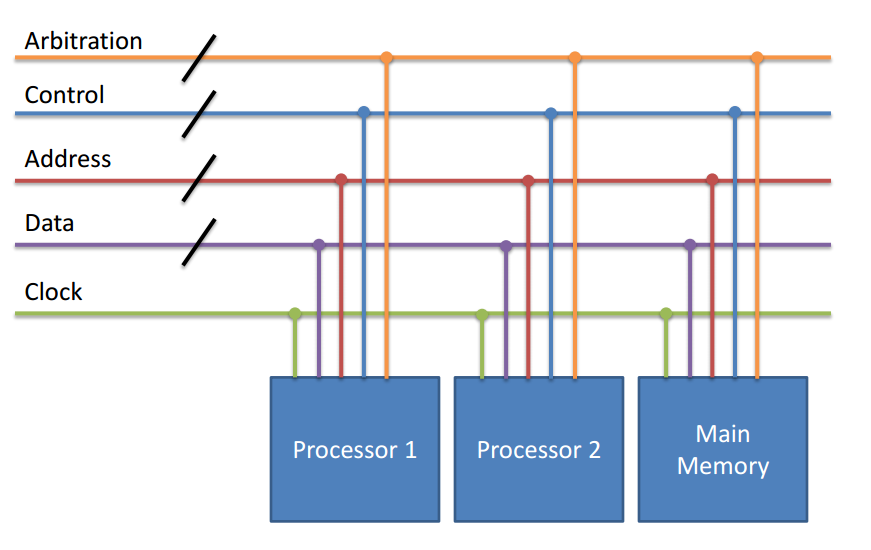
\includegraphics[width=1\textwidth]{img/bus_primatives.png}
    \caption{Primitive Multi-Drop Memory Bus }
    \cite{ComputerArchCoursera}
    \label{fig:bus_primative}
\end{figure}
Computer Bus which is the primitive version of the inter-connection network was designed to transfers data between components inside a computer, or between computers. They are defined to include all computer hardware components and software, included with communication protocols, in order to communicate devices. Devices is generally called as node or end node in taxonomy. However, this definition is quite broad and it covers from today's Internet network to cloud computing network and evolved in many aspect to different direction.

In figure \ref{fig:bus_primative}, There is an early multi-drop bus example. Multi-drop bus term is used for a bus line with many element on a line (not a ring), and there is an arbitration mechanism, so it is normal computer buses which is used in interconnection taxonomy. The multi-drop buses includes 5 separated wires which is distinguished by their purpose. Arbitration line decide actually how has right to speak, request. There is a logic devices to determine the arbitration and it is one of the most crucial research area in computer architecture and especially interconnector design\cite{hennessy2012computer}. Control wire is actually determine the purpose of the node. Generally, they are $store$ and $load$ operations. The address wire determine the requested address from corresponding place, in this case there is no cache controller so directly memory. Data wire carries the data which is stored or load, so the communication is synchronous, with consecutively request and reply. Lastly, clock wire provides a fixed, constant frequency to carry values.\cite{hennessy2012computer}

On recent systems the communication mechanism between nodes are quite more complicated comparing with given primitive example. The pace in the development on parallel systems makes correlation and communication between notes chaotic. Systems comprise with many nodes and requires high bandwidths  to overcome and increase their bottleneck. Intercommunication is still the slowest part of mainframe and personal computers. On the other hand, with multi layer memory aspect, communication between nodes and parallel computing gets more and more complicated. It makes every cache controllers a member of interconnector and perhaps  more. Today, there are some coherent interconnector which are also responsible with traffic management (i.e. QoS), barriers between devices and memories, and coherency\cite{armcoherentinterconnector}.

\begin{figure}[h!]
    \centering
    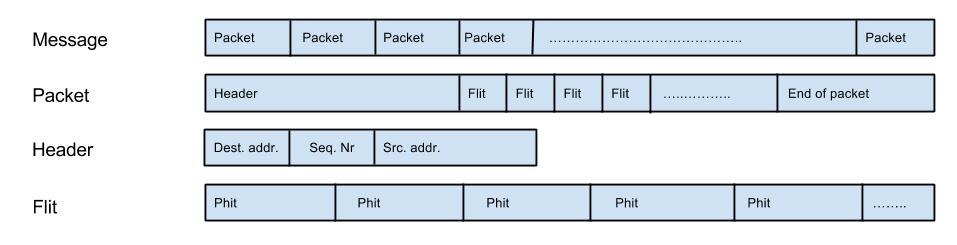
\includegraphics[width=1\textwidth]{img/Message_Anatomy.jpg}
    \caption{An example of interconnector message anatomy }
    \label{fig:message_anatomy}
\end{figure}

There are two main category of computer interconnectors which are host based On-Chip and System/Storage area network and remote over LAN and WAN networks inter-connectors. On-Chip networks purpose to mitigate the on-flight latency and chip-crossing wire delay problems related with increased technology scaling and transistor integration. Nevertheless, there is not enough space in a single chip to fill many cores. It is a good design for interconnecting ALU, registers caches, compute tiles, and perhaps several cores and memory. System/Storage area networks are the most used interconnection systems between multi-processors, multi-computer, multi-thread systems and memory system interconnection between this cores. Because of physically constrains such as distance and density, it is usual the interconnector between systems and their I/O extensions (e.g DMA chips). LAN and WAN based systems are actually designed to connect enormous number of node together. This kind of networks distributed several locations and interconnecting PCs cluster of computers. Cloud computing is actually one of the good example to show the ability of this species. On of the other advantage of remote interconnectors is that they are generally build on well-known protocols which are tested and acknowledged protocols e.g. Ethernet, GSM, IP, TCP, UDP. All routing issues are tested for many years and solved properly.\cite{hennessy2012computer}.

Modern interconnections with advance switching and routing mechanism are using message protocols.  In figure \ref{fig:message_anatomy}, an example of simple interconnector message anatomy is shown. Alternatively, the bus anatomy we mention above, the message based protocols are packetized. However, this packetizing process has some overhead as latency\cite{ComputerArchCoursera}. Message anatomy of interconnectors comprises several layers\cite{0122007514}.
\begin{description}
\item[Message]The message is the unit of information which must be transmitted with a propose. If it is about cache coherency, It could be whole line of the cache to provide coherency.
\item[Packet]Packets are the fixed maximum sized  smallest unit of information which include routing information in its header section. It can also include sequence number for flow control protocol. Its size is depending on the arbitration mechanism on the router or switches. It comprises with data flits which actually part of information in message.
\item[Flit]The small unit of link layer is called flit. Flits size are depending on the switching algorithms. In circuit switching flit size are whole packed. They are typically 4 byte to 16 byte.
\item[Phit]It is the unit of the physical layer in the interconnectors design. Its size is depending on the clock cycle of the interconnector. On the primitive bus example, the clock mechanism determine the phit size when it tick. They are around 8 bit to 32 bit.
\end{description}
 In order to characterize interconnector device we will use several feature of networks which are switching mechanism, switching mechanism, routing algorithms, topology, and flow control of networks. These feature are determine depending on application domain and defuse all character of network. Across the designs, performance with latency and bandwidth parameters and queuing theory is the valuable analysis tools to define network and its classification\cite{hennessy2012computer}.
\todo[inline] put the quotes of interconnection networks appendix E questions here.
\subsection{Topology}
Topology is a mathematical study of shapes and the points and their relationships in the environment. Network topology is actually determining the path and shape of the network. The shapes which topology concerns depending on the dimension they are build on. Electronic circuit are generally build on two or tree dimensional space. The wire and nodes are the basic element of interconnector topologies, but also router is the switch element which can decide the path. The node could be grouped to regulate communication and bandwidth e.g. there could be two group as memories and processors. Also, there are two main type of network topologies, that are In-directly connected distributed and directly connected centralized. The root of "central" word in telecommunication comes from this switches, but they are too vast topics to discuss in this thesis. The basic idea of the centralizing topology is to use a central switching fabric between nodes. The switching fabrics is actually external subsystem or combination of systems, e.g omega and crossbar network topologies\cite{0122007514}.

\begin{figure}[h!]
    \centering
    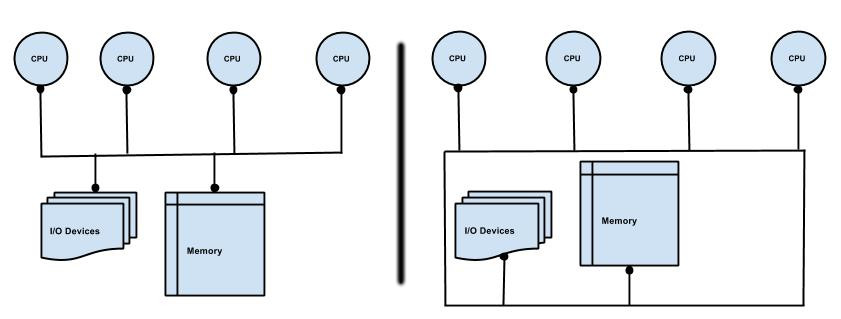
\includegraphics[width=1\textwidth]{img/busandring.jpg}
    \caption{A) Bus topology example B) Ring topology example}
    \label{fig:busring}
\end{figure}
 The general assumption of topologies is wire are faster then logical routers and transactions.-Today, there is in chip transaction devices which are faster then wires\cite{hennessy2012computer}.- In order to design efficient topology, optimum cost and measure its quality, we have several parameters, which are diameter of tomography, routing distance, minimum bisection bandwidth and degree of a node.
\begin{description}
  \item[Routing Distance] It is any given two points distance by mean of number of links or hops
  \item[Diameter] It is maximum routing distance between any two point of the network. In figure \ref{fig:busring} and example A, it is from the first node of the bus to last node, so it is 5. It could be sometimes not that obvious, but it is the most far two nodes' distances.
  \item[Average Distance] Average Distance is $TotalDistance/NumberofNodes$. It is one of the value which using in average latency calculation. Generally performance values are compared with each other by average latency.
  \item[Minimum Bisection Bandwidth] If network is segmented in two equal part, and if the bandwidth of these two segments is as minimum as possible, it is called minimum bisection bandwidth. Typically, this bisection will be the most occupied lines, and the bandwidth of bisection will effect total performance sharply. To embody it better, it is like a bridge between two island. Most of the traffic caused by the occupation on the bridge in ordinary traffic networks. The inner island bandwidth is futile to effect overall traffic.
  \item[Degree of a Node] It is the properties of each node to imply how many nodes it is directly connected to. The node with the highest degree is applied as degree of the network.
\end{description}
\begin{figure}[h!]
    \centering
    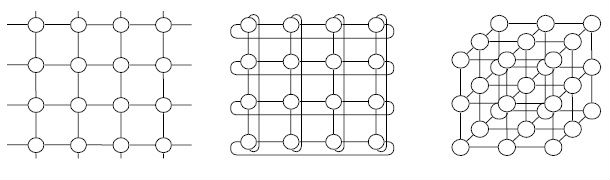
\includegraphics[width=1\textwidth]{img/multidimensional.jpg}
    \caption{A) Mesh topology example B) Torus topology example C) 3D mesh  topology example\cite{HPCfigure}}
    \label{fig:meshestorus}
\end{figure}
The number of topologies designed in literature can be too many to count, but the idea behind them has always same logic. Topology directly effect performance, but also greatly impact the cost of systems. Physical constrains such as chips' pin-out, light speed, dimension count on the board and etc. determine topologies properties. Generally chips are reducing their inner bandwidth, when they are communicating with out side of chip, due to the restriction of building pins\cite{hennessy2012computer}.
\subsection{Topologies}
\begin{description}
\item[Buses and Rings] Buses and rings are the first dimensional primitive and basic type of interconnector topologies. They are both directly connected nodes in in sequence as shown in figure \ref{fig:busring}, but rings are end around buses. Namely, ring topology aims to reduce the longest link which is actually diameter of the network. If $N$ is the total number of node, node $i$ is directly connected to node $i+1$, and node $i-1$ except element $0$ and element $N-1$ in buses, and in rings, every node $i$ is directly connected to every node $i+1$ and $i-1$ in mod $N$.  In bus topology, diameter is $N-1$, in ring topology, diameter is $(N-1)/2$. In segmented and pipelined networks, rings are also increasing bandwidth, because when 2 closer nodes communicate with each other, other nodes can connect over all around the line. For example, When 4 and 5  is communicating, in buses, there is no way from 1, to 6 but in rings there is another links goes around the network to connect 6 and 1, so bisection bandwidth is 2 in rings and 1 in buses Rings looks more efficient and logical to use it, however, in practice it could be hard to implement because of the physical constraints, but they are vast topics to discuss in this section.
\item[Two Dimensional Networks: Meshes, Tori] Meshes and Tori are the idealized structure of two dimensional interconnectors, because every best two dimensional forms to connect $m^2$ nodes. while mesh topology is derivative of bus topology, tori are derivative of rings-as showed in figure \ref{fig:meshestorus}, so terminologies uses meshes end around term instead of torus. The bisection bandwidths are $2\sqrt{N}$ for meshes and $4\sqrt{N}$ for tori. The diameters are $2\sqrt{N}-2$ for meshes and $\sqrt{N}-1$. Degree of the network is 4(5 in some terminologies), and every nodes degree is same in the torus network which can be seen in figure \ref{fig:meshestorus}.\cite{ComputerArchCoursera}
\item[Multiple Dimensional Networks] They are excessive versions of the mesh and torus networks which are influenced by the chips packaging technology. Multi dimensional system over 2D space is still good to obtain higher bandwidth and balance the traffic but more complicated example are seen with Storage/System, local and wide area networks. Because they are instead of chips real 3D systems and surely, 3D networks works better in 3D systems. On an $N$ dimensional system, if you want to build more dimensional systems such as $N+1$ or $N+i$, it increase the wire length exponentiation when you increase $i$. Wire length is related with flight time of the data, and it effects directly bandwidth. One of the idealized for of the multi dimensional networks are cubes. Cubes are the three dimensional topologies which every nodes are 3Th degree and all nodes are equally close to each other. In figure \ref{fig:meshestorus}, there is an example of three dimension mesh. CM1 and Thinking machine is the examples of their practice today in market. They actually connects thousands of computers in hyper cube topologies. They connects the mesh dimensions, which are two dimensional with each others.
\todo[inline]{formalize the diameters, bisection bandwidth}
\item[Fully Connected Star] Fully connected stars are directly connected star topologies which actually known in some terminologies as mesh networks. This topology is the best possible topology which have been designed so far, because every nodes are directly connected with each other within $1$ routing distance. If there is $N$ number of node that means the bisection bandwidth is exactly $1024$, because each node has for every other nodes another links with an other bandwidth, it makes it bottleneck-less topology.
\item[Omega and Fat Tree] Omega and fat tree topologies are examples of centralized systems. They are improvements of crossbar switches. Crossbar switches are expensive designs because its complexity increase quadratically with the number of ports. Instead of the increasing the design complexity, it increase the stages\ thus, permutation\cite{hennessy2012computer}. With $N$ number of node and with $kxk$ switches, $log_{k}N$ stages each of which contains $N/k$ is required in omega network. However, the reduction of the implementation cost has some negative sides, which are lower bandwidth, dropped packet, more latency.
\todo[inline]{formalize the diameters, bisection bandwidth and a bit more about fat tree}
\end{description}
\subsection{Switching}
\todo[inline]{I could add figures about switching later also latency calculation formula could be attacked here or latency part.}
Switching name root originally comes from circuits. It is complex combination of many circuits switch which actually connects conductors together. It determines in interconnection networks how data is allocated for data transmission, i.e. how and when the input channel will be connected to the output channel. Buffer states, channel flow, and surely routing algorithms effects the switching designs as we know so far from computer network design. To sum up, it is actually model how to connect different locations and nodes together\cite{ComputerArchCoursera}.
\begin{description}
\item[Circuit Switching] Circuit switching is the oldest type of communication model. Most of the telecommunication networks still using its advantages. Circuit switching reserve whole line and its whole its bandwidth during communication. It could be advantage, if message is infrequent and long, e.g. analogue sound transfer. In addition to this, message could be whole part instead of fixed sized packets, phits, and flits. On its implementation, there are two state which are circuit establishment phase and message transmission phase\cite{0122007514}. The physical path between point $A$ and point $B$ is reserved before it started to transfer message. The line is reserved through $routing probe$ message. It is generally one phit and one fhit long message. It discover the route which is provided by router algorithms and invoke routers to preserve corresponding line to the packet destination. When $routing probe$ reached to the destination note, it means all intermediate router(switches) reserved for connection, then point $B$ will sent back acknowledgment message and finish the establishment. This establishment is tricky point in circuit switching, because it requires setup delay which actually comprises with logical calculation time and time of flight. This time is called as RTD(Round trip delay) or RTT(Round trip time), and it is one time delay. There is no routing decision and switching delay. That is good for long message, but disadvantage for short message. At the end of the communication, it must be ended with $reset probe$.
\item[Packet Store and Forward Switching] This Switching method is packetizing type of communication model. It divides each message into the fixed length packets and phits and flits. Each channel(output and input) in every switches has its reserved buffer memory as large as packet size. It stores fits and plits in this buffers until they are totally loaded, and switch them to the right output channel. The most important think of packet switching is every packets are switched(routed) individually from the source to the destination. In addition to this, every packets could be routed through different switches and routers depending on routing algorithms. If there are parallel routers between source and destination nodes, it could makes calculation of the chaotic, so they are not preferred by real-time systems' network. Also, implementation of buffers and switching each packets again and again continuously makes it slower and expensive. However, on the other side, it has many advantages. When we need to communicate with short and frequently packets, we can not reserve whole line for two nodes. It makes the same line provide many nodes with sending small packets and also dynamic routing is what makes our Internet works today. Theoretically, It does not have establishment state, but piratically it is so usual to implement it upon link layer.
\item[Packet Cut Through] It is also called as wormhole networks. It is a hybrid combination of circuit and packet store switching. It allows simple, small, cheap, and relatively fast switches. In theory, it does not need any buffer and instead of waiting the tail of the message, it just start routing the packet from the head. In implementation input channels could use buffer memories, because of busy output channels, and it whole message could get stalled if there is no buffer to store it, then it need to demand this message again, or worse, it could perhaps lose whole packets forever. In implementation, it divides packets flits and phits and intercept header of packets and then continuously switch or route all phits or flits.
\end{description}
\subsection{Routing}
Routing of the networks is actually predetermined set of rules which draw the path of the packets they will follow on networks. Namely, routing algorithms determine the path over network topology with using switching mechanisms. If we look at the smaller picture, each intermediate router on the network determines which input port is to be connected to which output port. Some of the routing algorithms can complexly adapt their algorithms depending on the network condition i.e. they can monitor bandwidth and latency differences, compare them with demands and route depending on latest traffic, and some of the can simply choose random available path. However, there are two significant criteria of ideal routing: They should be dead-lock free, and they should give the shortest path.
\begin{description}
\item[Deterministic Obvious Routing]
\item[Non-Deterministic Obvious Routing]
\item[Adaptive Routing]
\end{description}
\subsection{Flow Control}

